\section{Introduction} %\label{sec:extenstion_introduction}

This chapter extends the previous work in \cite{calderon_scalable_2023}. In many applications, there is a need to support overlay DCEL operations when the input contains complete polygon data (as is the case in the previous chapter) with polygons that may contain two new types of edges, namely, ``dangle" and ``cut" edges. Here, we extend the overlay DCEL approach to accept scattered and noisy line segments as input, rather than being restricted to clean polygon data. This enhancement builds on the scalable polygonization methods presented in \cite{abdelhafeez_ddcel_2023}, enabling the overlay of real-world datasets composed of vast sets of line segments —datasets that existing techniques are unable to process effectively. The proposed solution is an extension of the approach we used in Chapter \ref{sec:methods}, for handling polygons with holes.

Figure \ref{fig:extension_dcel_example} illustrates the fundamental components of a DCEL including the two new types of special half-edges. \textit{Dangles} are half-edges with one or both endpoints not incident on another half-edge endpoint; both half-edge $\overrightarrow{fj}$ and its twin are considered dangle edges. \textit{Cut-edges} are half-edges connected at both ends that do not form part of any polygon. The half-edge $\overrightarrow{dg}$ and its twin are classified as cut-edges.

\begin{figure}
    \centering
    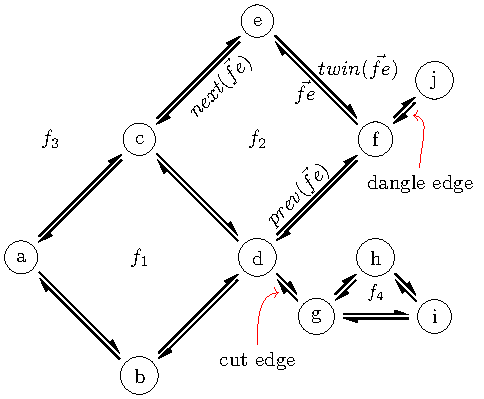
\includegraphics[width=0.6\linewidth]{chapterExtension/dcel_example2}
    \caption{Components of the DCEL structure with dangle and cut edges.}\label{fig:extension_dcel_example}
\end{figure}

The remainder of this chapter is organized as follows. Section \ref{sec:extension_methods} describes the polygon extraction process for adapting line segment inputs, which extends the overlay method to support dangle and cut edges. In Section \ref{sec:extension_experiments}, we present additional experiments to quantify and assess the performance of the proposed polygonization on datasets with large volumes of line segments.
